% !TEX program = pdflatex
\documentclass{article}
\usepackage{pgfplots}
\pgfplotsset{compat=1.18}
\begin{document}
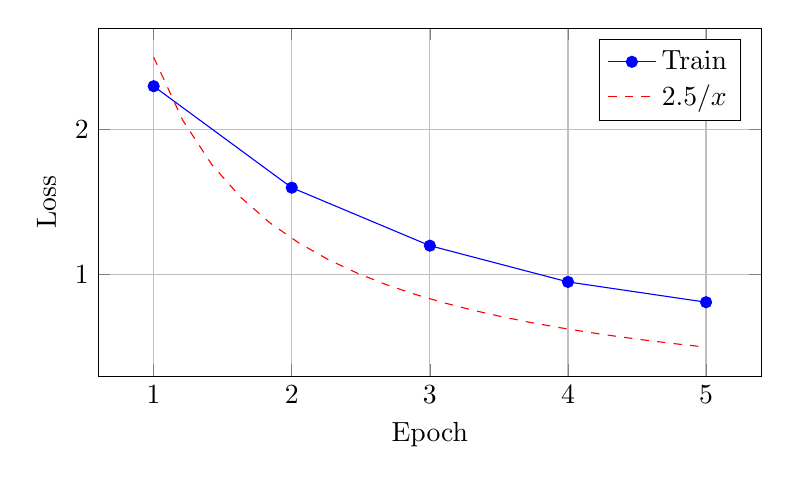
\begin{tikzpicture}
\begin{axis}[xlabel={Epoch},ylabel={Loss},legend pos=north east,grid=major,width=10cm,height=6cm]
\addplot[blue,mark=*] coordinates {(1,2.3) (2,1.6) (3,1.2) (4,0.95) (5,0.81)};
\addplot[red,dashed,domain=1:5,samples=20] {2.5/x};
\legend{Train,$2.5/x$}
\end{axis}
\end{tikzpicture}
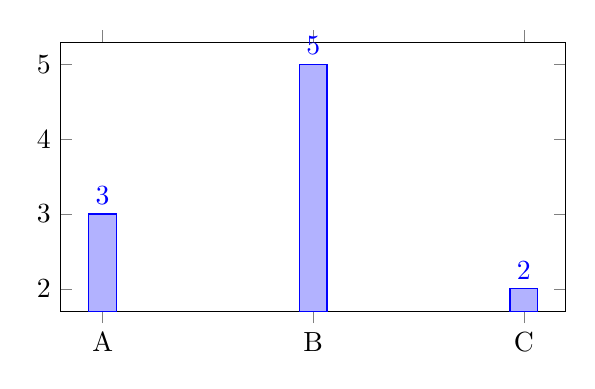
\begin{tikzpicture}
\begin{axis}[ybar,symbolic x coords={A,B,C},xtick=data,nodes near coords,width=8cm,height=5cm]
\addplot coordinates {(A,3) (B,5) (C,2)};
\end{axis}
\end{tikzpicture}
\end{document}
